\chapter{Methods}\label{sec:methods}

The entirety of the research for this thesis is performed with pen and paper and a computer running the Linux operating system Ubuntu. The programming language Python, with its very intuitive syntax and large libraries for scientific computing and plotting, was used for the calculations and most of the plots for this thesis. More specifically, the open-source QuTiP library\textsuperscript{5} for Python was used to create the Bloch sphere plots. All function plots were embedded directly into \LaTeX  by using the pgfplots package\textsuperscript{6}.

\footnotetext[5]{The open-source QuTiP library for Python may be downloaded from \url{http://qutip.org/}}
\footnotetext[6]{The \LaTeX  pgfplots package may be downloaded from \url{https://www.ctan.org/pkg/pgfplots}}

For the implementation of the quantum kNN algorithm there are two fundamentally different ways: Running it a) by simulating a QC or b) by actually executing it on a real QC. The required tools for both possibilities will be explained in the following subsections.

\section{Liqui$\ket{}$}
\label{subsec:simulation}

Classical computers can be used to simulate the behaviour of small quantum computers. Such simulations are associated with exponential computational costs thereby limiting the number of simulated qubits. Since current state-of-the-art quantum technology uses around ten qubits, a classical computer can still be used for simulation.

For the quantum computing simulations in this thesis the quantum simulation toolsuite Liqui$\ket{}$ developed by Microsoft Research will be used. Liqui$\ket{}$ is based on the functional programming language F\# and allows for simulation of up to 30 qubits \cite{liquid}. It comes with a large palette of predefined single and multi qubit quantum logic gates and allows for custom-defined quantum gates such as nCNOT and rotation gates controlled by $n$ qubits which is crucial for some of the work done in this thesis. A short piece of example code from Liqui$\ket{}$ written in F\# is shown in Fig.~\ref{fig:liquidsnippet}.

\begin{figure}[H]
      \centering
       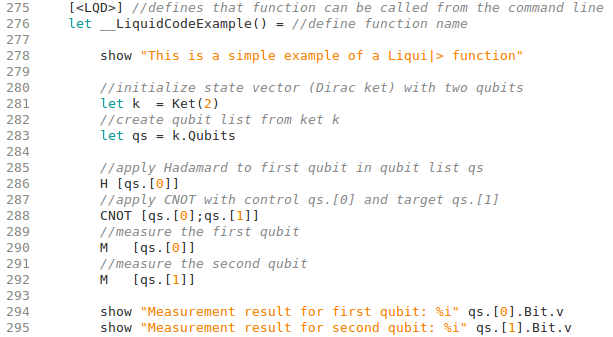
\includegraphics[scale=0.55]{img/liquidcodesnippet.png}
       \caption{\label{fig:liquidsnippet} F\# code snippet from Microsoft's quantum simulation toolsuite Liqui$\ket{}$}
\end{figure}

A Lenovo ThinkPad T450 containing an Intel i5 processor with 2 cores and 8GB random-access memory (RAM) is used for all quantum simulations in this thesis.

\section{IBM Quantum Experience}
\label{subsec:ibmqc}

Earlier this year IBM has enabled public cloud access to their experimental quantum processor containing five non error-corrected superconducting qubits located at the IBM Quantum Lab at the Thomas J Watson Research Center in Yorktown Heights, New York \cite{ibmquantumcomputer}. Instead of only simulating on classical hardware, this opens up the possibility of executing the QML algorithm on actual quantum hardware.

The so-called IBM Quantum Experience provides the user with access to the "Quantum Composer" which is the main tool for algorithm design. The quantum composer shown in Fig.~\ref{fig:composer} consists of 5 horizontal lines, one for each qubit, and enables the user to choose from a universal gate set (bottom of Fig.~\ref{fig:composer}) consisting of 10 quantum logic gates. 

DISCUSS THE AVAILABLE GATES HERE!

Additionally, there are two different measurement types: a) A measurement in the standard z-basis ($\ket{0}$ / $\ket{1}$) resulting in a probability distribution over all possible states and b) a Bloch measurement that visually projects the state onto the Bloch sphere. The user can compose an algorithm by applying up to 40 quantum logic and measurement gates to the five qubits by means of drag-and-drop.

\begin{figure}[H]
      \centering
       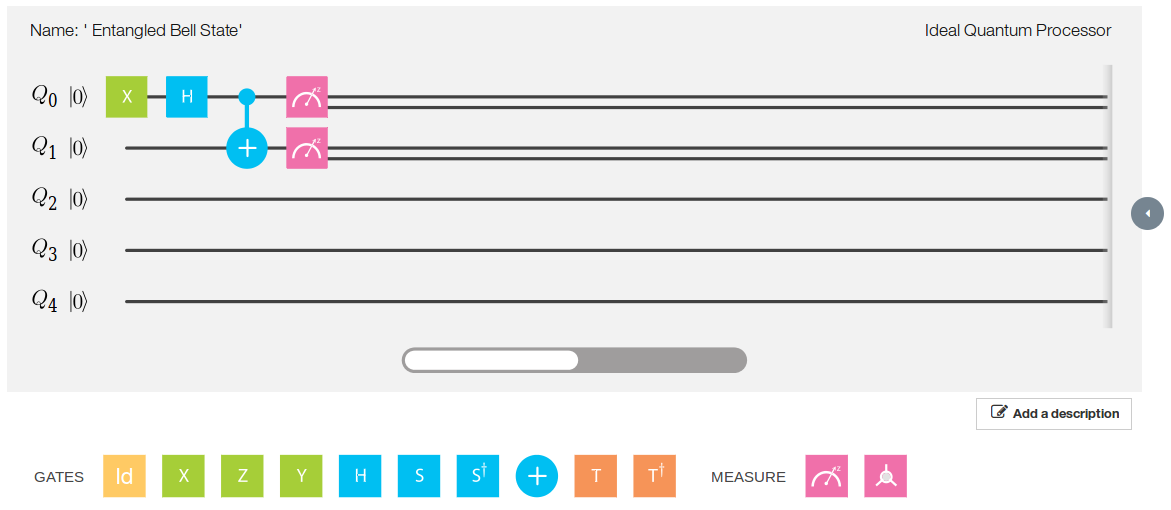
\includegraphics[scale=0.36]{img/ibmcomposer.png}
       \caption{\label{fig:composer} Screenshot showing IBM Quantum Composer}
\end{figure}

By spending limited user coins the gate sequence of a composed algorithm is then send to IBM's QC in New York and depending on the waiting queue and the availability of the QC the results will be sent back via mail within a few minutes or days. IBM Quantum Experience also allows for free quantum simulations under ideal or real conditions which provides a great tool for experimentation without spending user coins.

The main limitation of the IBM Quantum Experience are the qubit decoherence times since they restrict the maximum number of possible operations before the qubits lose their quantum behaviour and their quantum information. Thus, the number of quantum gates is currently limited to only 40 which essentially means 39 logic gates and 1 measurement gate. According to the qubit calibration results shown in Fig.~\ref{fig:calibration}, the amplitude damping times of the five qubits range from \SI{52.3}{\micro\second} to \SI{81.5}{\micro\second}. Furthermore, the phase damping times range from \SI{60.9}{\micro\second} to \SI{112.4}{\micro\second}. Currently, the implementation of a single qubit quantum logic gate takes 130ns and applying a CNOT gate takes 500ns \cite{ibmgatetimes}.

\begin{figure}[H]
      \centering
       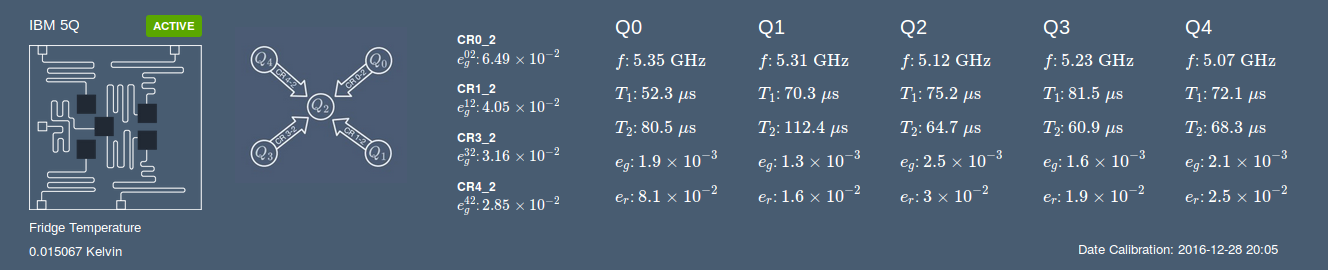
\includegraphics[scale=0.33]{img/ibmcalibration.png}
       \caption{\label{fig:calibration} Screenshot of IBM QC calibration results (28. December 2016 - 20:05)}
\end{figure}
